\chapter{Architettura riusabile per backend di Protelis}
\section{Piattaforme di simulazione}
L'architettura utilizzata per Protelis si dimostra flessibile, adatta alla
portabilità su diversi sistemi reali\cite{Clark2015} e simulati quali
Alchemist\cite{alchemist} (Figura 3b) e NASA World Wind\cite{Bell2007}.

L'architettura utilizzata per Protelis si dimostra flessibile, adatta alla
portabilità su diverse piattaforme. Per fare ciò è necessario realizzare un
backend che definisca i meccanismi di comunicazione tra i dispositivi e
gestisca l'esecuzione della macchina virtuale Protelis.

% TODO: Descrizione di alchemist migliore
\subsection{Alchemist}
\begin{figure}
  \centering
  % 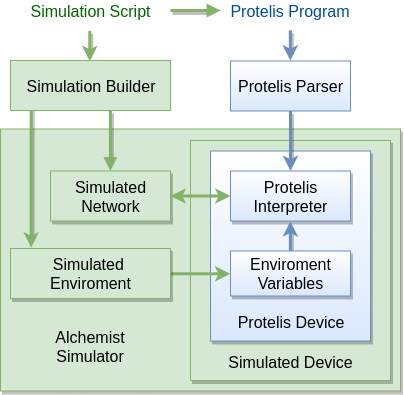
\includegraphics[height=5.5cm]{media/alchemist-architecture.png}
  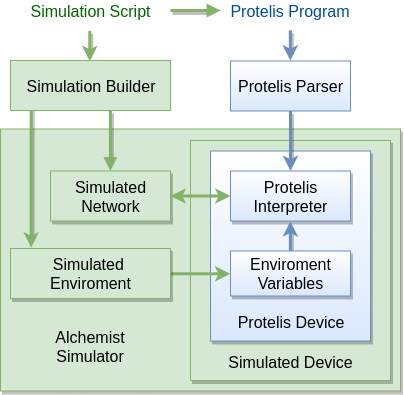
\includegraphics[width=0.7\linewidth]{media/alchemist-architecture.png}
  \caption{Implementazione di Protelis utilizzata in Alchemist}
\end{figure}
Tra le realizzazioni esistenti l'esempio più rilevante è
Alchemist\footnote{https://alchemistsimulator.github.io/}: un simulatore per
computazione pervasiva, aggregata e ispirata alla natura. Esso utilizza al
proprio interno un meta-modello nel quale dispositivi vicini e interconnessi
comunicano seguendo un insieme di leggi ispirate al mondo della chimica.

Alchemist prevede la probabilità di utilizzare incarnazioni, ovvero
implementazioni concrete del proprio meta-modello per modellare uno specifico
concetto di interesse. Una di queste incarnazioni è quella che consente al
simulatore di eseguire un programma Protelis all'interno della propria
infrastruttura, che permette di creare e gestire una rete di nodi simulati
(Figura /ref{fig:alchemist-architettura}).

\subsection{NASA World Wind}
NASA World Wind\footnote{https://worldwind.arc.nasa.gov/} è un progetto
open-source cross-platform sviluppato dalla NASA, che offre un'interfaccia di
programmazione per creare, in maniera rapida, delle visualizzazioni 3D
interattive di un globo virtuale. Si differenzia da altri software simili come
Google Earth\footnote{https://www.google.it/intl/it/earth/} perché non è una
semplice applicazione, piuttosto un'intera SDK che può essere utilizzata come
base per costruire una propria applicazione.

È stato utilizzato per dimostrare come Protelis possa essere uno strumento che
permette di controllare anche dispositivi reali come uno sciame di droni. In
questa
simulazione\footnote{https://github.com/Protelis/Protelis-Demo-Visualized} 25
quadricotteri, disposti a griglia, volano a qualche centinaio di metri da
terra. Essi fanno uso di comunicazione a corto raggio, 500 metri, per parlare
con i dispositivi adiacenti.

% TODO: Spiegare bene la parte del CodePath
\section{Sistemi distribuiti}
I costrutti fondanti della programmazione aggregata e i building block possono
semplificare notevolmente il design e lo sviluppo di applicazioni in un contesto
di Internet-of-Things\cite{DBLP:journals/computer/BealPV15}. Infatti consente di
costruire, tramite composizione delle proprie API, delle applicazioni
distribuite robuste e affidabili.

Un sistema distribuito è una collezione di computer indipendenti che appare
all'utente finale come un unico sistema coerente\cite{tanenbaum2016}.  Il
concetto di indipendenza comporta che i dispositivi appartenenti al sistema non
hanno risorse condivise, in particolare la memoria; allo stesso tempo questi
devono raggiungere un obiettivo comune. Deve essere quindi prevista una modalità
in cui questi componenti possano comunicare, per scambiarsi informazioni o
coordinarsi.

Al fine di eseguire macchine virtuali Protelis in un contesto distribuito è
necessario implementare un modello di scambio di messaggi tra queste.
L'architettura di Protelis (\ref{subsec:Architettura di Protelis}) è stata ideata avendo questo problema ben chiaro,
pertanto è possibile estenderla facilmente, tramite l'implementazione di uno
strato middleware, che si occupa ciò.

% Serializzazione:
% - time efficient
% - hashing (probabilità molto bassa di errore)
%

% TODO: API Protelis qui o in architettura?
\section{Architettura riusabile}
% Perché? A che bisogno risponde?
%
% Introduzione classi di Protelis
% Strategy per Speaker e NetworkManager
% Definizione di Device e DeviceCapabilities
% Definizione modello riusabile
